
%%% Preamble

\documentclass[	DIV=calc,%
							paper=a4,%
							fontsize=11pt,%
							twocolumn]{scrartcl}	 				% KOMA-article class

\usepackage[english]{babel}										    % English language/hyphenation
\usepackage[protrusion=true,expansion=true]{microtype}				% Better typography
\usepackage{amsmath,amsfonts,amsthm}					            % Math packages
\usepackage[pdftex]{graphicx}									    % Enable pdflatex
\usepackage[svgnames]{xcolor}									    % Enabling colors by their 'svgnames'
\usepackage[hang, small,labelfont=bf,up,textfont=it,up]{caption}	\usepackage{float}
% Custom captions under/above floats
\usepackage{epstopdf}												% Converts .eps to .pdf
\usepackage{subfig}													% Subfigures
\usepackage{booktabs}												% Nicer tables
\usepackage{fix-cm}													% Custom fontsizes
%\usepackage{apacite}                                                % Apa citations
\usepackage[hyphens]{url}
\usepackage{hyperref}
\usepackage[nosectionbib,numberedbib]{apacite}
%\usepackage{graphicx}
\graphicspath{ {./images/} }
\usepackage{pdfpages}
\usepackage{pgffor}
\AtBeginDocument{\renewcommand\refname{Bibliography}}
\bibliographystyle{apacite}
\raggedbottom


%%% Custom sectioning (sectsty package)
\usepackage{sectsty}													% Custom sectioning (see below)
\allsectionsfont{%															% Change font of al section commands
	\usefont{OT1}{phv}{b}{n}%										% bch-b-n: CharterBT-Bold font
	}

\sectionfont{%																% Change font of \section command
	\usefont{OT1}{phv}{b}{n}%										% bch-b-n: CharterBT-Bold font
	}



%%% Headers and footers
\usepackage{fancyhdr}												% Needed to define custom headers/footers
	\pagestyle{fancy}														% Enabling the custom headers/footers
\usepackage{lastpage}	

% Header (empty)
\lhead{}
\chead{}
\rhead{}
% Footer (you may change this to your own needs)
\lfoot{Bartosz Czapski - D10123621}
\cfoot{}
\rfoot{\footnotesize \thepage}	% "Page 1 of 2"
\renewcommand{\headrulewidth}{0.0pt}
\renewcommand{\footrulewidth}{0.4pt}



%%% Title, author and date metadata
\usepackage{titling}															% For custom titles

\newcommand{\HorRule}{\color{DarkGoldenrod}
									  	\rule{\linewidth}{1pt}
										}
%%begin novalidate
\pretitle{\vspace{-30pt} \begin{flushleft} \HorRule 
				\fontsize{20}{20} \usefont{OT1}{phv}{b}{n} \color{Black} \selectfont 
				}
\title{Analysis and Evaluation of Functionality of RAFT Consensus Algorithm in Internet of Things Domain }					% Title of your article goes here
\posttitle{ \end{flushleft}}

\preauthor{\begin{flushleft}
					\large \lineskip 0.5em \usefont{OT1}{phv}{b}{sl} \color{DarkRed}}
\author{Bartosz Czapski - D10123621 }										
\postauthor{\footnotesize  \usefont{OT1}{phv}{m}{sl} \color{Black} 
                    \par
					TU060 - MSc in Computer Science (Advanced Software Development) - Technological University Dublin 
					\par Starting date: \textcolor{red}{01/02/2022} All exams passed
					\par 1st attempt \textcolor{red}{(Revised)}
					\par Data set for this research will be gathered during the experiments
					\end{flushleft}\HorRule}

					
%%end novalidate
\date{}																				% No date


%%% Begin document
\begin{document}
\maketitle
\thispagestyle{fancy} 			% Enabling the custom headers/footers for the first page 

\section{Background, Context and Scope}
Consensus is regarded as the primary problem which, once solved, will enable implementation of fault-tolerant distributed system \cite{Lamport2005GeneralizedCA}. Distributed systems merge with Internet of Things (IoT) creating decentralized system of collaborating Smart Objects(SOs) which sense, store, and interpret information from surrounding environment and act on their own, cooperate with each other exchange information with other kinds of IoT devices, or client nodes \cite{7488250}.\begin{figure}[H]
\centering
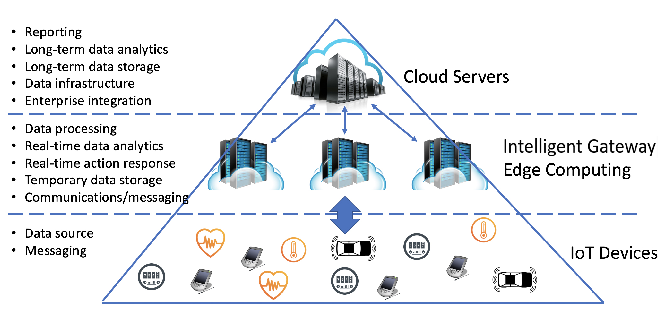
\includegraphics[width=0.45\textwidth]{images/edge.png}
\caption{Layer architecture of edge computing-based IoT}\shortcite{8123913}
\end{figure}
\noindent Consensus algorithms enable collection of machines to cooperate as a coherent group, able to  survive the failures of some of its members. This feature warrants consensus algorithms to  play a key role in building reliable large-scale distributed systems \cite{10.5555/2643634.2643666}.\smallskip \newline Multiple authors recently focused on the idea of distributed consensus algorithms, their application in IoT domain \cite{BOF2017601,RAGHAV2020101291,whittaker2020matchmaker,ZHANG2020574,FORTINO202034}, and implementation of self-organizing real-time systems architecture \cite{10.1007/978-3-030-30278-8_34,GUERRERO2019131,7372286}.\smallskip \newline Distributed consensus algorithms, when adopted for IoT, provide  mechanism for balanced decision making on the edge nodes, and avoiding losing data from IoT devices in the presence of a number of malfunctioning devices by improving the robustness and reliability of the decision process \cite{6740862}.
\section{Problem Description}
A consensus algorithm is used to attain, in distributed and multi-agent systems, overall system reliability in the presence of a number of faulty processes, or involving multiple unreliable nodes. When discussed in the context of IoT, consensus algorithm is required to achieve fast event ordering, predictable delivery time and minimal packet loss rate in edge computing networks.\smallskip \newline Current approach to consensus between the nodes in IoT domain  includes modifying existing consensus algorithms: blockchain \cite{ WANG2020101871,10.1007/978-3-030-30278-8_34}, cooperative game model \cite{GULATI2020102222}, proportional-integral-derivative (PID) \cite{SHI201873}, developing new algorithm \cite{8737532}, or using revised Paxos consensus algorithm \cite{10.5555/3324320.3324322, Cachin2010YetAV}.\smallskip \newline Raft algorithm achieves consensus via an elected leader. Raft cluster is built of leaders and followers, and a node in a cluster can be either leader, or follower (in case of unavailability of the leader, follower becomes candidate and undergoes election process). Raft uses heartbeat messages to implement leader – followers’ relationship, where each of the followers expects heartbeat from leader within the timeout frame. Election process start when message is not received within time limit, otherwise timeout is reset \cite{10.5555/2643634.2643666}.
\begin{figure}[H]
\centering
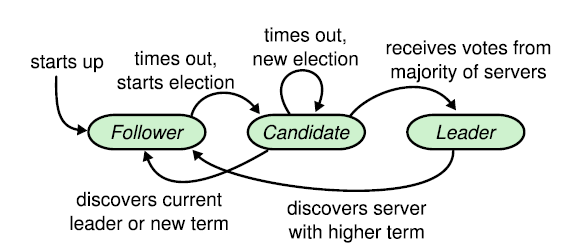
\includegraphics[width=0.45\textwidth]{images/raft_alg.png}
\caption{RAFT protocol}\shortcite{10.5555/2643634.2643666}
\end{figure}
\noindent Raft has an advantage over the other consensus algorithms, noticeably Paxos, that its understandability is greatly improved \cite{UCAM-CL-TR-857}. As of date of writing this paper, author is unaware of Raft algorithm being used in distributed IoT architecture for achieving consensus among the edge nodes.
\subsection{Approaches to solve the problem}
Recent works discuss various consensus methods that are applicable to IoT  networks. Below is the selection of most interesting propositions of solving consensus problem within IoT domain.\smallskip \newline \shortciteA{10.1007/978-3-030-30278-8_34} proposed decentralized self-balancing architecture that implements consensus algorithm with an aim to improve usage of all IoT devices on the network, and resilience to disconnection while providing increased privacy and security. In their work, authors focused on small number of devices and missed the opportunity to test their architecture with different consensus algorithms against multiple use cases.\smallskip \newline \shortciteA{6740862} designed a distributed consensus algorithm with the goal of improving decision making at the edge nodes of IoT, with a focus on global consensus of multiple services. As per authors’ suggestion, more focus should be given to research on collaborative methods for the realization of information exchange and resource allocation in IoT environment.\smallskip \newline Similar attempt to develop Distributed Resource AssiGnment and OrchestratioN (DRAGON) algorithm is presented in the paper authored by \shortciteA{8737532}. Authors tested proposed algorithm within the scope of two use cases focusing on  its convergence and performance properties.\smallskip \newline  \shortciteA{Hao2018EdgeConsAE} proposed a novel consensus protocol, EdgeCons, for achieving fast event ordering in edge distributed systems, and although primary results are very promising authors have to design proper monitoring of the system. Additionally, timeframe of recovery of EdgeCons ``leadership share`` can take interminable amount of time.\smallskip \newline Byzantine Fault (BFT) consensus algorithm  is adapted by \shortciteA{GRAMOLI2020760} for blockchain technology, and distributed systems. This algorithm, practical BFT (pBFT), achieves clear consensus in each round of operation and cannot be manipulated.\smallskip \newline \shortciteA{GULATI2020102222} presented different approach with implementing Weighted Voting Game (WVG) model for conflict resolution in argumentation enabled social IoT networks. Authors simulated and evaluated proposed model’s performance within one use case scenario. Additionally, authors notice that implementing model in multi-agent environment to enable agreement among conflicting agents is very promising future work.\smallskip \newline Meritocratic mechanism is the base for \shortciteA{FORTINO202034} the Friendship and Group Formation (FGF) algorithm designed with  organization and improvement of IoT objects collaboration in mind. Authors of the paper could extend the research by implementing additional use cases with multiple agents cooperating.\smallskip \newline  \shortciteA{OROSTICA201915} discussed distributed multi-cast algorithm for robust average consensus over internet of things environments. Proposed algorithm was tested and compared with  Push-Sum-Based algorithm introduced by \shortciteA{BOF2017601} that implemented asynchronous communication between the nodes on the network. Oróstica and Núñez mentioned that their algorithm outperformed Bof et al. algorithm, but missed the opportunity to compare it with additional consensus algorithms.\smallskip \newline \shortciteA{10.1145/3132211.3134454} discussed the problem of distributed placement algorithm for  ad-hoc optimization in Mobile Edge Computing. They developed algorithm for solving the online version of the placement problem, based on an iterative matching process, which achieved good performance during experiments. As results presented in the paper are very promising, authors did not attempt to implement proposed algorithm in ‘real-life’ multiple scenarios, and focused on online single use case simulation only.\smallskip \newline It is worth mentioning work of \shortciteA{CUI20204349} on positive edge consensus of nodal networks, where authors presented consensus algorithm addressing the issue of consensus in complex networks. It is not directly related to IoT environments but has a potential as ``computationally cheaper especially for large-scale systems.``\smallskip \newline \shortciteA{ROCHA20191} proposed successful model of scalable architecture for discovering and managing group of IoT devices. Whereas their model is successful, it does not take into account impact of devices’ energy consumption, or increase in number of nodes connected. \smallskip \newline \shortciteA{SALIMITARI2020100212} compared multiple blockchain based consensus methods that can be applied to IoT networks. They did not achieve implementation satisfying all challenges listed in the paper. \smallskip \newline \shortciteA{7776972} presented a survey advances in consensus of Multi-Agent Systems (MAS), but as they pointed out ``survey is far from an exhaustive literature review and there may still be some important results missing in the review due to space limitation.``\smallskip \newline Similarly, \shortciteA{6810888} and \shortciteA{7339456} proposed distributed algorithms that are utilising MAS properties (consensus and invariant summation of state variables) for Economic Dispatch Problem (EDP) which could have interesting applications for IoT architecture.\smallskip \newline \shortciteA{8638200} introduced consensus techniques that provide a complete information about network status by implementing one case study using the consensus aggregation within Fog environments.\smallskip \newline \shortciteA{7417252} developed algorithms for sensing resource discovery in IoT with their main focus on gossip policy. Paper did not discuss implementation of other communication protocols (e.g., asymmetric, or coordinated broadcast).\smallskip \newline  \shortciteA{MONDAL202041} discussed the optimal topology problem and way of solving it using Genetic Algorithm (GA) technique to achieve optimal adjacency matrix. Authors came to conclusion that their research can be extended by including more agents in the experimental network by changing the dimension of adjacency matrix.\smallskip \newline \shortciteA{RAGHAV2020101291} proposed proof of elapsed work and luck (PoEWAL) consensus algorithm for satisfying security requirements (e.g., integrity, authentication, and availability) on IoT devices. Although PoEWAL was compared with other consensus algorithms in terms of consensus time, energy consumption, and network latency authors missed the opportunity to make it more complete by not including scalability, computing requirements and decentralization features.\smallskip \newline Similarly, \shortciteA{whittaker2020matchmaker} compared multiple consensus protocols (e.g., Paxos, Matchmaker Paxos  and Raft), and applied them to IoT universe, focusing on applying proactive reconfiguration in elastic systems.
\subsection{Gaps in Research}
Although there is extensive body of research in the field of consensus algorithms, and their application for IoT architecture author of this paper noticed that not all avenues are properly explored. One common gap that emerges is the research is the lack of the ‘real-life’ scenarios \cite{GULATI2020102222,10.1145/3132211.3134454} and inadequate number of use cases tested \cite{10.1007/978-3-030-30278-8_34, 8737532,FORTINO202034,MONDAL202041}. Another important issue is the absence of proper monitoring \cite{Hao2018EdgeConsAE} , and missed opportunity to discus consensus with nodes scalability in mind \cite{6740862, ROCHA20191,RAGHAV2020101291}. While some of papers discussed provided good comparison of multiple algorithms, most fall short from the comprehensiveness perspective \cite{OROSTICA201915, SALIMITARI2020100212,7417252}. One avenue, that is of particular interest, is the implementation of Raft consensus algorithm for the purpose of minimising latency and packet loss on IoT network in the face of multiple node failures, and contrasting the results with those of Paxos and pBFT algorithms \cite{whittaker2020matchmaker,GRAMOLI2020760}.
\section{Research Question}
Can implementation of Raft consensus algorithm in IoT network decrease latency on the network in the presence of malfunctioning edge nodes when compared to Paxos consensus algorithm?
\section{Hypothesis}
The objective of this research is to implement, analyse and evaluate performance of Raft consensus algorithm on IoT network in the presence of multiple node failures. As current research on the topic of consensus problem in IoT domain does not discuss, nor benchmark Raft, author will attempt to provide performance measurements (latency, faulty nodes discovery and packet loss rate) in the presence of number of malfunctioning devices. Additionally, results of the above experiment will be compared against the results of Paxos algorithm.\smallskip \newline Author of this research will conduct experiment where original (non-existent) data will be collected, and different consensus algorithms will be compared on IoT network to confirm H1 and H4. Quantitative (numerical) data from the experiment will be collected and analysed, and provide definitive result. Exhaustive answers will be provided by comparing quantitative data, author will test and confirm an existing theory. 
\smallskip \newline \textbf{Null hypothesis H\textsubscript{0}:} Implementation of the Raft consensus algorithm will not improve latency of the IoT network in the presence of faulty edge nodes.\smallskip \newline \textbf{Alternative hypothesis H\textsubscript{1}:} Implementation of the Raft consensus algorithm will significantly improve latency of the IoT network in the presence of faulty edge nodes.\smallskip \newline \textbf{Alternative hypothesis H\textsubscript{2}:} Implementation of the Raft consensus algorithm will increase discovery of the faulty edge nodes in the IoT network.\smallskip \newline \textbf{Alternative hypothesis H\textsubscript{3}:} Implementation of the Raft consensus algorithm will decrease packet loss rate in  in the IoT network.
\smallskip \newline \textbf{Alternative hypothesis H\textsubscript{4}:} Implementation of the Raft consensus algorithm will outperform Paxos consensus algorithm.
\section{Design and Implementation}
Below table represents planned activities for this this research.   
\begin{figure}[H]
\centering
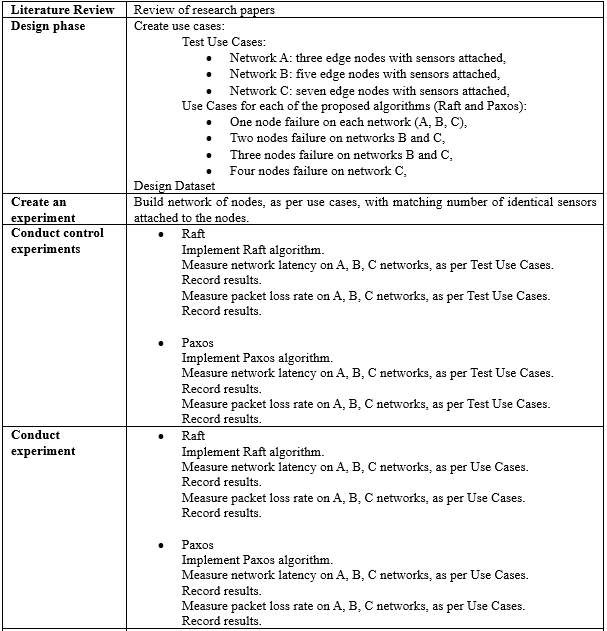
\includegraphics[width=0.45\textwidth]{images/taskAndObj.png}
\caption{Tasks and Objectives to test hypothesis}
\end{figure}
\noindent During the Literature review phase additional information regarding the research problem is hoped to be revealed. Design phase will establish use cases that will be followed during the experiments. As this research problem include comparison of efficiency of different algorithms, use cases will be divided in two categories: test use cases and use cases.\smallskip \newline Test use cases are planned to be implemented during the control experiment where three networks are created: A, B and C. Network A consists of three IoT nodes, Network B of five IoT nodes, and Network C of seven IoT nodes.
\begin{figure}[H]
\captionsetup{font={color=red}}
\centering
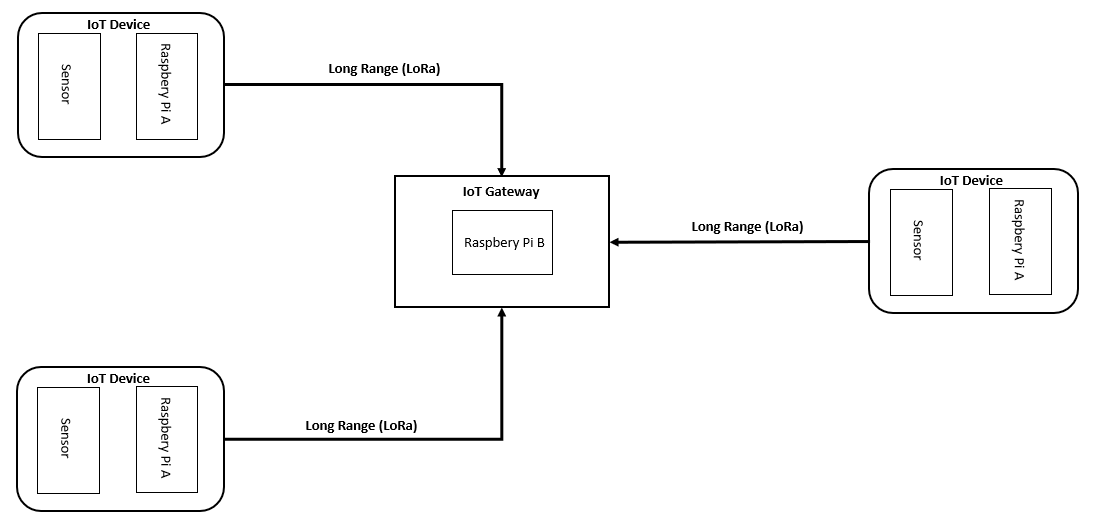
\includegraphics[width=0.45\textwidth]{images/arch_diagram.PNG}
\caption{Example of three node network with gateway}
\end{figure}
\noindent Third-generation Raspberry Pi (RPP) 3 Model A+ single board computer (SBC) will serve as an IoT edge node. It features a Broadcom BCM2837B0, Cortex-A53 (ARMv8) 64-bit SoC @ 1.4GHz quad-core processor System on a Chip (SoC), 512MB LPDDR2 SDRAM, 2.4GHz and 5GHz IEEE 802.11.b/g/n/ac wireless LAN and Bluetooth 4.2/BLE, Extended 40-pin GPIO header, Single USB 2.0 ports and Micro SD port. Raspberry Pi 3 Model A+ operates on 5V/2.5A DC power input. Sensor attached to each IoT node is \textcolor{red}{DockerPi Sensor Hub Development Board (EP-0106). It integrates various environmental sensors: temperature sensors, humidity sensors, air pressure sensors, lighting, and thermal imaging sensors.} Both, RPP and \textcolor{red}{DockerPi} sensor, will be connected using MB102 Breadboard with 3.3V 5V MB102 Breadboard Power Supply Module. Environmental data between sensors and nodes will be transmitted continuously. \textcolor{red}{Raspbery Pi 3 B will be used as IoT gateway}. Lenovo Ideapad 530s with 16GB of RAM and 8th gen Core i5 processor laptop \textcolor{red}{will be used for debugging}. \textcolor{red}{Connectivity between edge nodes and gateway will be established with TTGO Lora32 868/915mhz Sx1276 Esp32 Wifi Lora module.}
\begin{figure}[H]
\captionsetup{font={color=red}}
\centering

\includegraphics[width=0.45\textwidth]{images/components.png}
\caption{Components}
\end{figure}
\noindent Author of this paper chose Python programming language to implement Raft and Paxos algorithms. Python is widely used, and well documented programming language. Raspberry Pi SBC supports is natively. Additionally, Python libraries provide implementation of all two consensus algorithms.\smallskip \newline During the control experiment \textcolor{red}{Packet Error Rate (PER) and} Round-Trip Time (RTT) between the client and edge note, and packet rate will be measured in networks A, B and C. Control experiment will be repeated for each algorithm. \textcolor{red}{The Raspberry Pi 3 B will act as an IoT gateway (receiver), receiving the environmental sensor data from the IoT devices, the cluster of Raspberry Pi 3 A with DockerPi Sensor Hub (transmitter) attached. The Raspberry Pi B will run a Python script, responsible for receiving, decrypting, and parsing the data payload from the sensor. Received data in JSON format will contain external temperature data,  onboard temperature data,  humidity data, light sensitivity data and pressure data. 
The dataset for this project will be constructed from transactions sent between the receiver and transmitters. Author will measure PER by counting the number of packets received by the IoT gateway out of a series of consecutive packets transmitted by the sensors. Additionally, author will attempt to measure RTT which can be defined as the amount of time it takes a packet to get from the transmitter to the receiver and back.}
\smallskip \newline Malfunctioning devices, as per use,  cases will be simulated by manually disconnecting Raspberry Pi SBC during the next Experiment stage. Planned use cases include: 
\begin{itemize}
  \item Failure of one node on networks A, B and C.
  \item Failure two nodes on networks B and C.
  \item Failure three nodes on networks B and C.
  \item Failure four nodes on network C.
\end{itemize}
\begin{figure}[H]
\centering
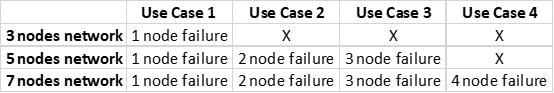
\includegraphics[width=0.45\textwidth]{images/use_cases.png}
\caption{Use cases}
\end{figure}
\noindent Data collected (RTT in milliseconds, and number of packet send between the nodes) during both phases, Control experiment, and Experiment will create dataset used for comparison of the efficiency of evaluated consensus algorithms \cite{Hao2018EdgeConsAE,721868}. The workload
will be capped to 1,000 events (sensor outputs) that will be transmitted on the path sensor-node-client, with their intervals evenly distributed to avoid any inconsistencies.     
\section{Evaluation}
Evaluation process will start with reviewing of data collected during the experiment.
\begin{figure}[H]
\centering
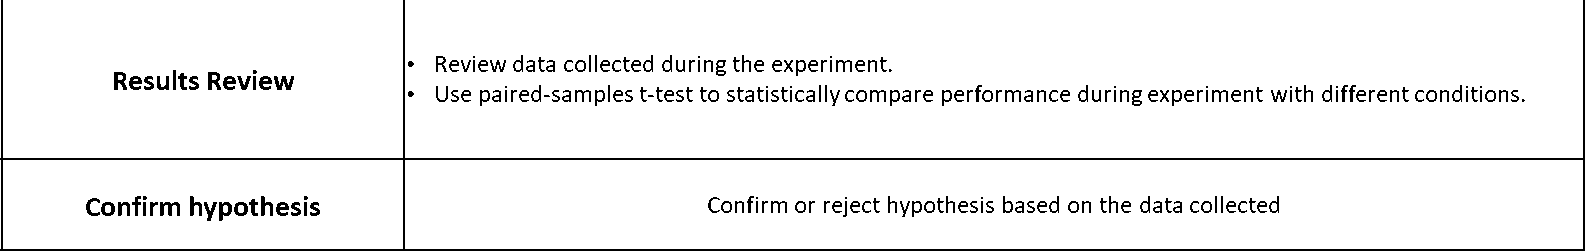
\includegraphics[width=0.45\textwidth]{images/bottom_taskAndObj.png}
\caption{Evaluation process}
\end{figure}
\noindent
T-test with paired-samples will be used to statistically compare performance of consensus algorithms during both experiments with different conditions. All RTT data collected during control experiment will be statistically compared to algorithms performances during research experiments.\smallskip \newline Proposed hypothesis H\textsubscript{1}, H\textsubscript{2}, H\textsubscript{3} and H\textsubscript{4} will be accepted independently based on the results achieved. Confirming of hypothesis H\textsubscript{1} and H\textsubscript{4} will confirm the research question.


%%\typeout{}

\bibliography{bibliography_file}

\section{Activities}
Below activities planned for this research are spread over the period of 13 weeks.
\begin{itemize}
  \item O1: Literature Review - 3 weeks
  \item O2: Design phase - 1 week
  \item O3: Create an experiment - 2 weeks
  \item O4: Conduct control experiment - 2 weeks
  \item O5: Conduct experiment - 3 weeks
  \item O6: Results Review - 1 week
  \item O7: Confirm hypothesis - 1 week
\end{itemize}
\clearpage
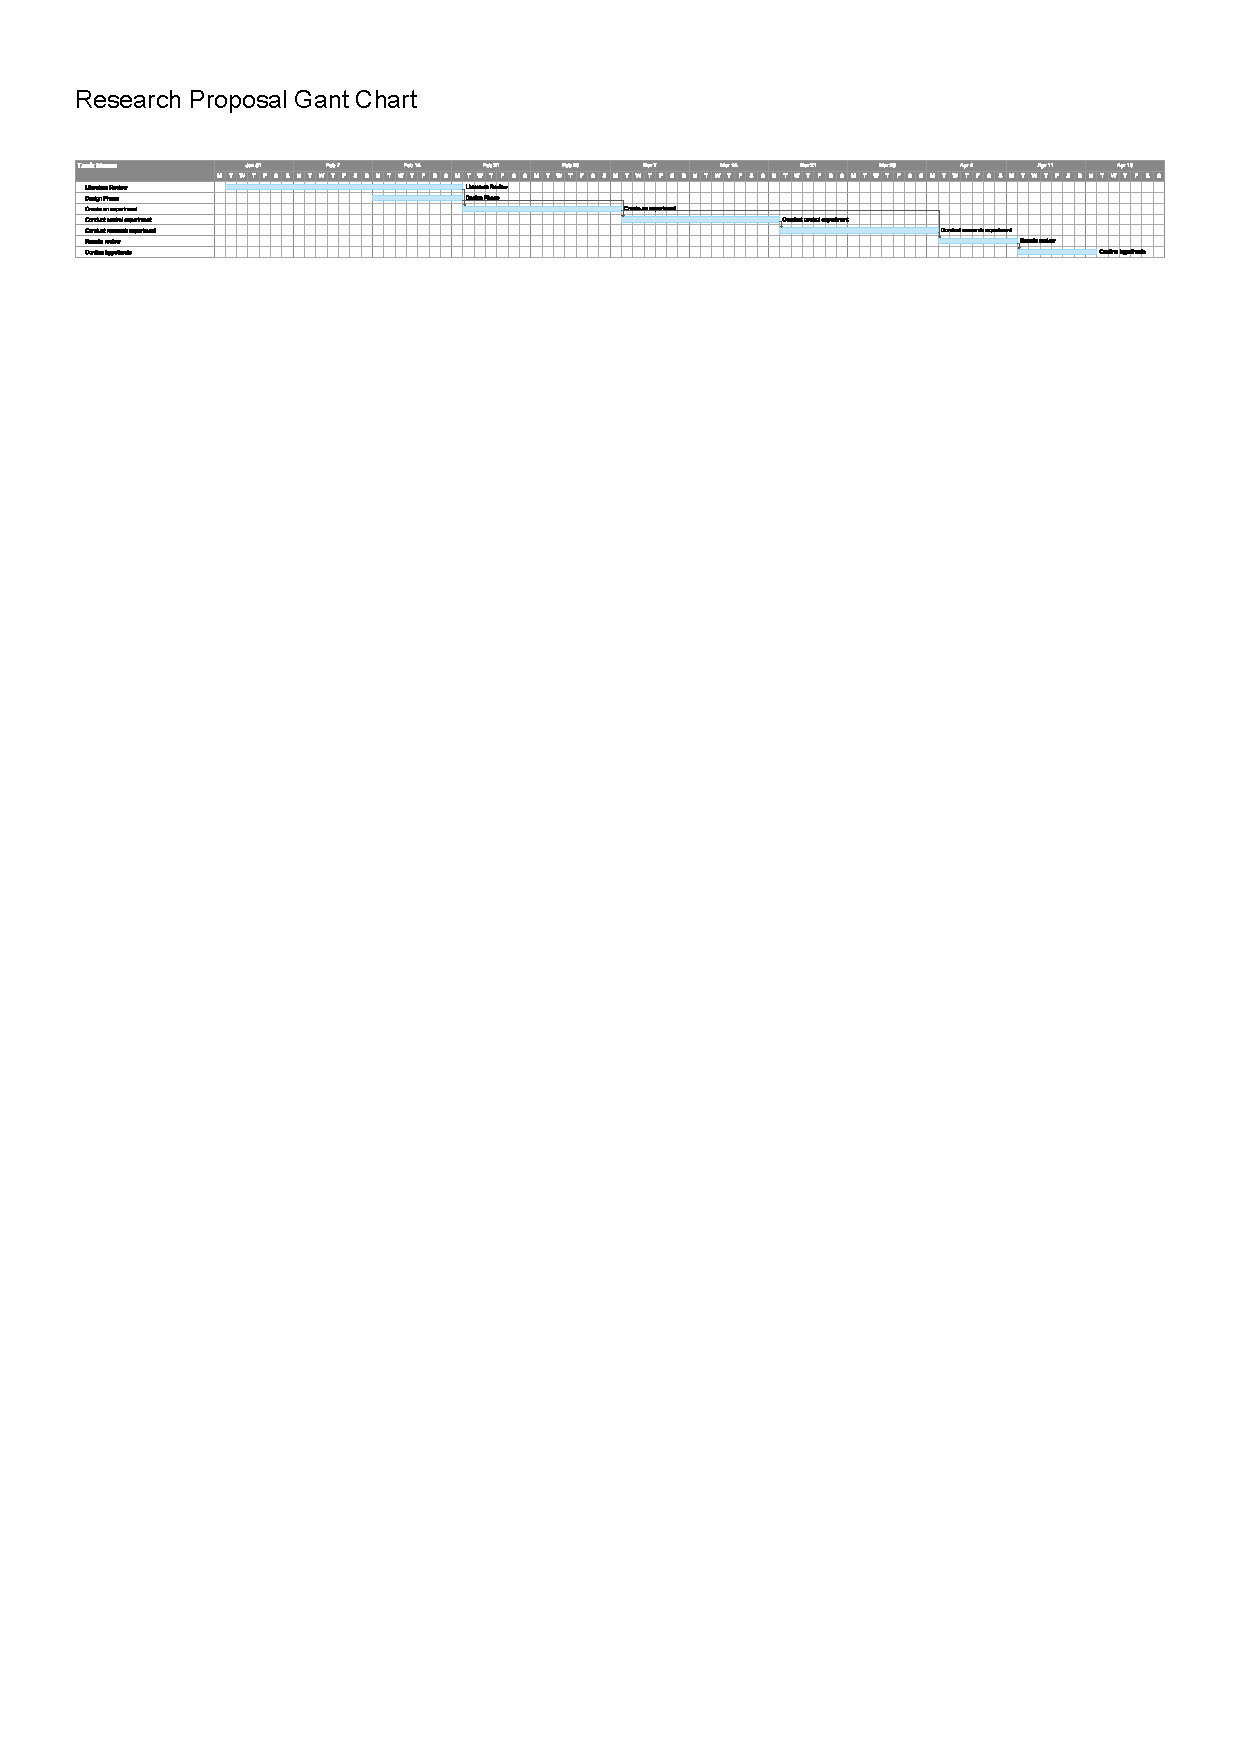
\includepdf[pages={1}]{pdfs/gant.pdf}


\section{Appendix}

\foreach \x in {1,...,8}
{%
\clearpage
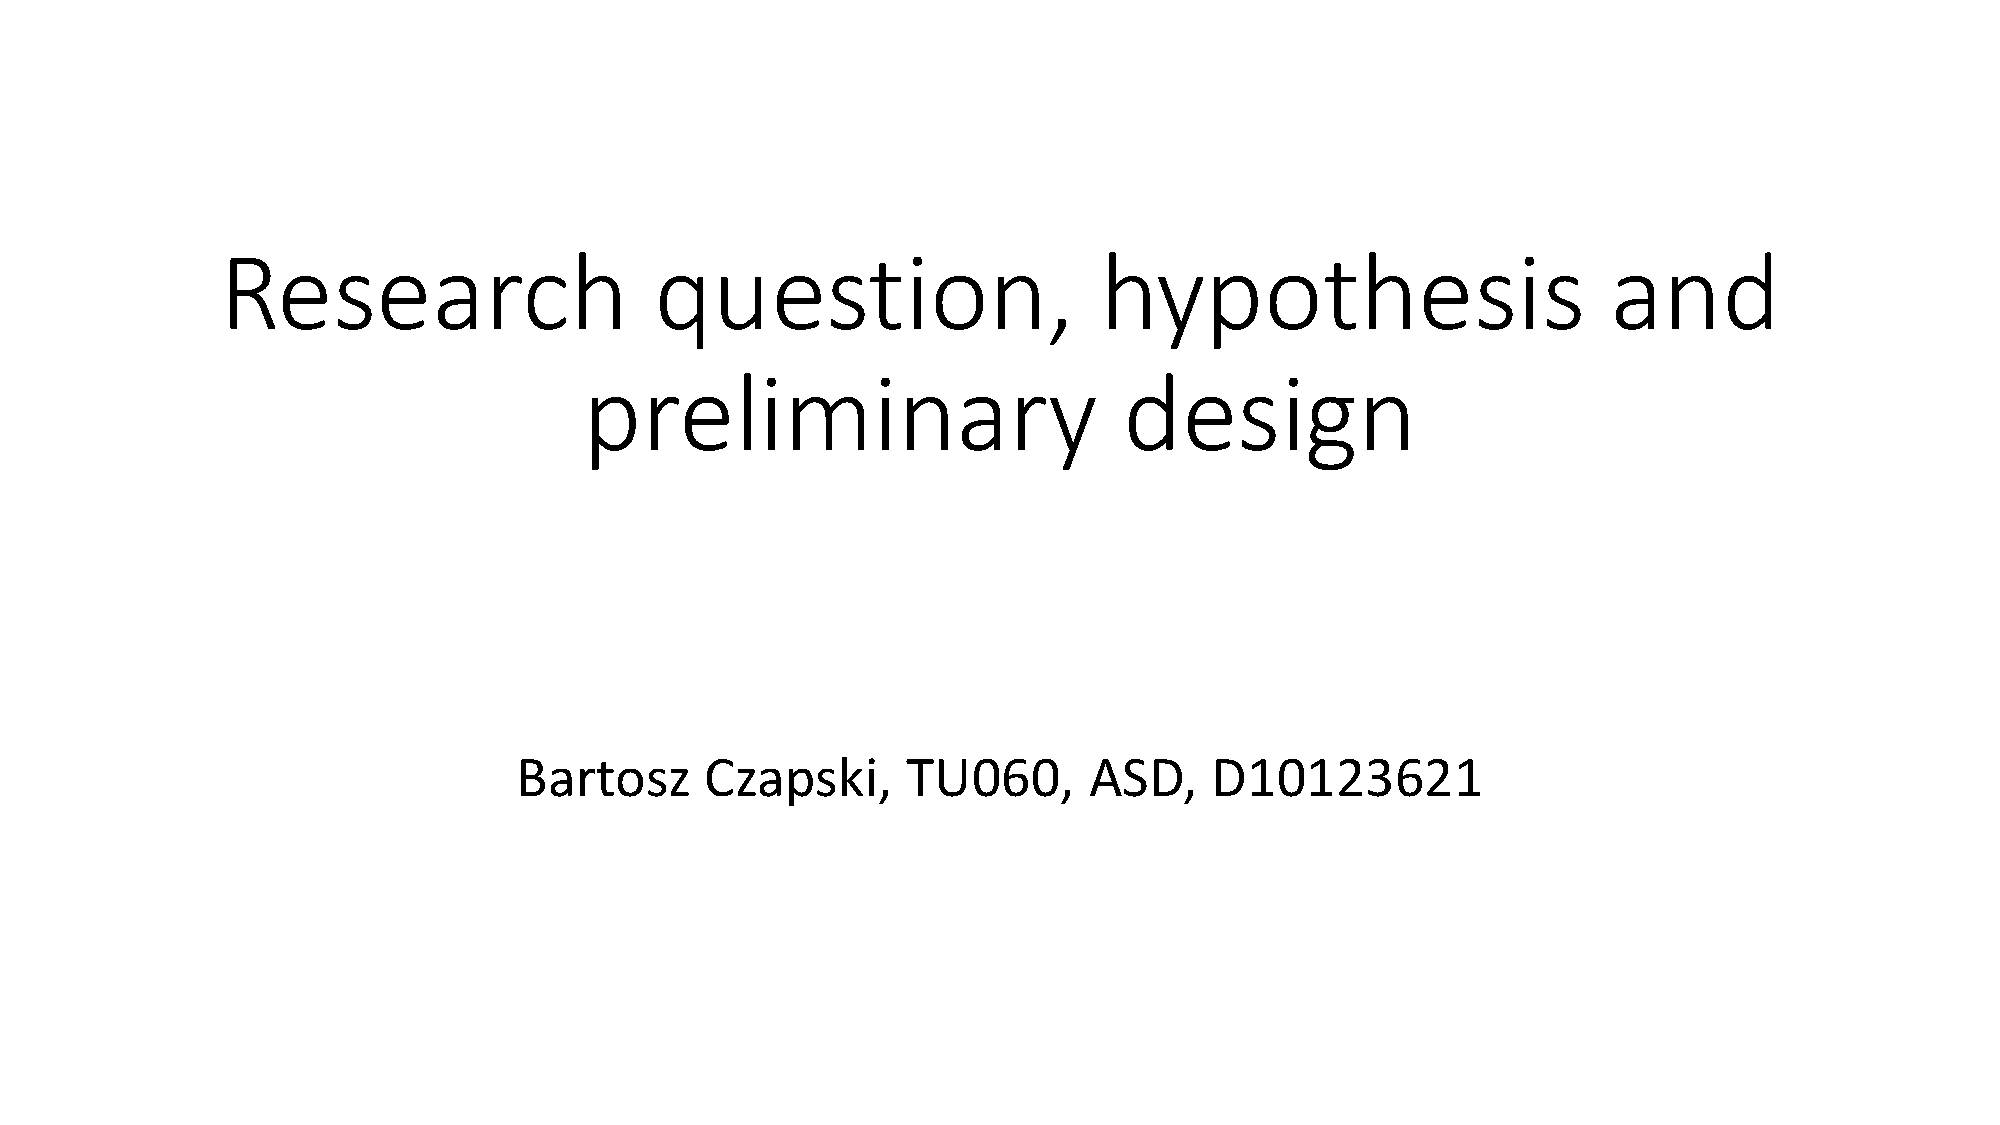
\includepdf[pages={\x}]{pdfs/D10123621_1.pdf}
}
\foreach \x in {1,...,8}
{%
\clearpage
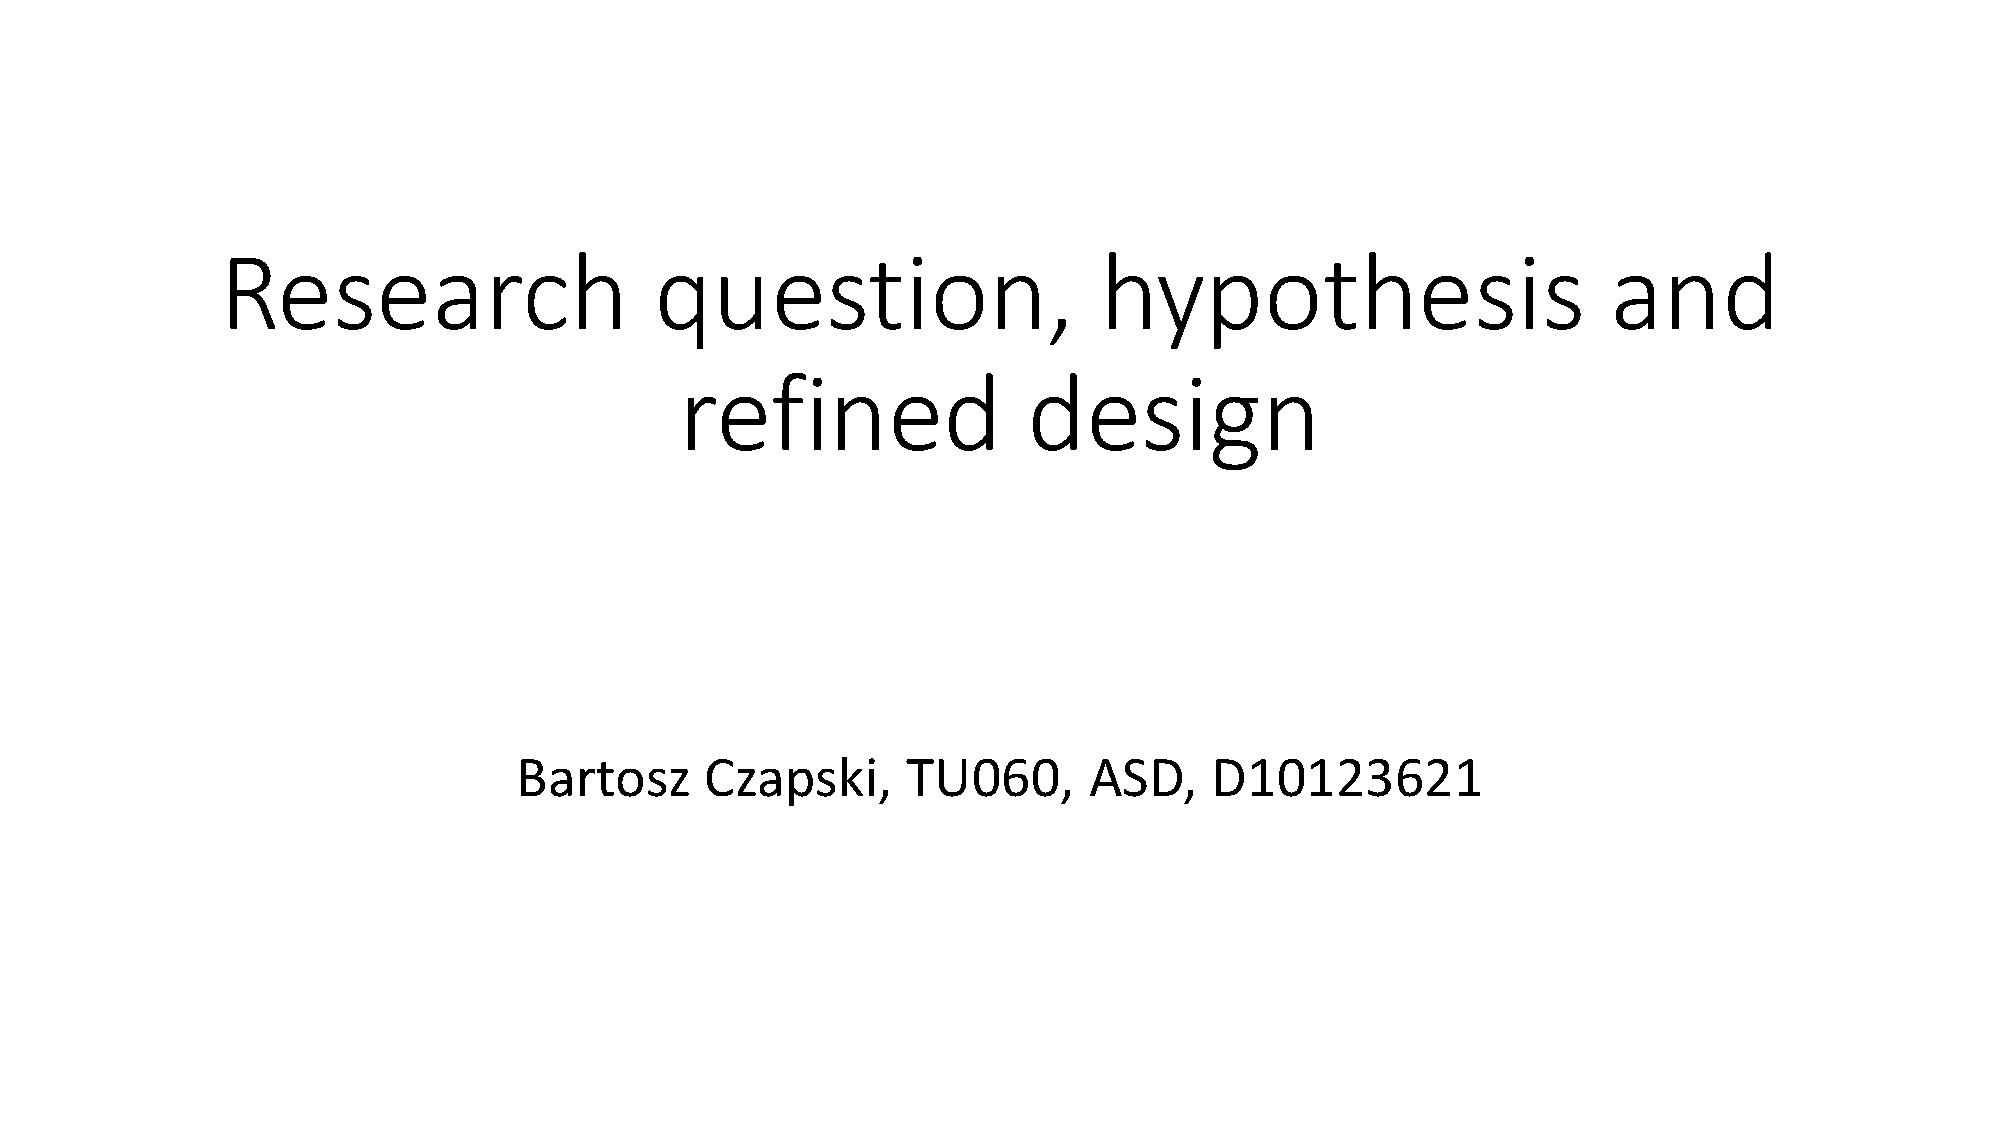
\includepdf[pages={\x}]{pdfs/D10123621_2.pdf}
}

\end{document}
